% ---------------------------------------------------------------------
% ---------------------------------------------------------------------
% ---------------------------------------------------------------------

\chapter[Modern techniques for the analysis of metabolomic data]{Modern techniques for the analysis of metabolomic data}
\label{chapter:modern_techniques}


% ---------------------------------------------------------------------
% ---------------------------------------------------------------------
\section{Projection based methods}
\label{projectionmethods}
In the previous chapter, the projection technique known as PCA has been introduced. As explained in section \ref{sec:PCA}, this method works by performing a dimension reduction to an original data matrix with dimensions $I \times J$, to a projected data matrix with dimensions $I \times M$, where $M<J$. Each new component of the projected data matrix is built trying to capture as much of the variability from the original data matrix as possible. So PCA is a projection technique that tries to reduce the dimensionality of the data while trying to maximize the information kept from the original data. This approach can be great for performing exploratory analysis of a data set or unsupervised analysis, but can be inefficient for performing supervised analysis such as regression or classification. The reason for this is that, while variables with the highest variability carry most of the information of the original data matrix, they do not have to be the ones able to explain the response we are trying to predict \parencite{kettaneh2005pca}. A conceptual explanation of this is presented in \autoref{figura02}.

\begin{figure}[htbp]\centering
		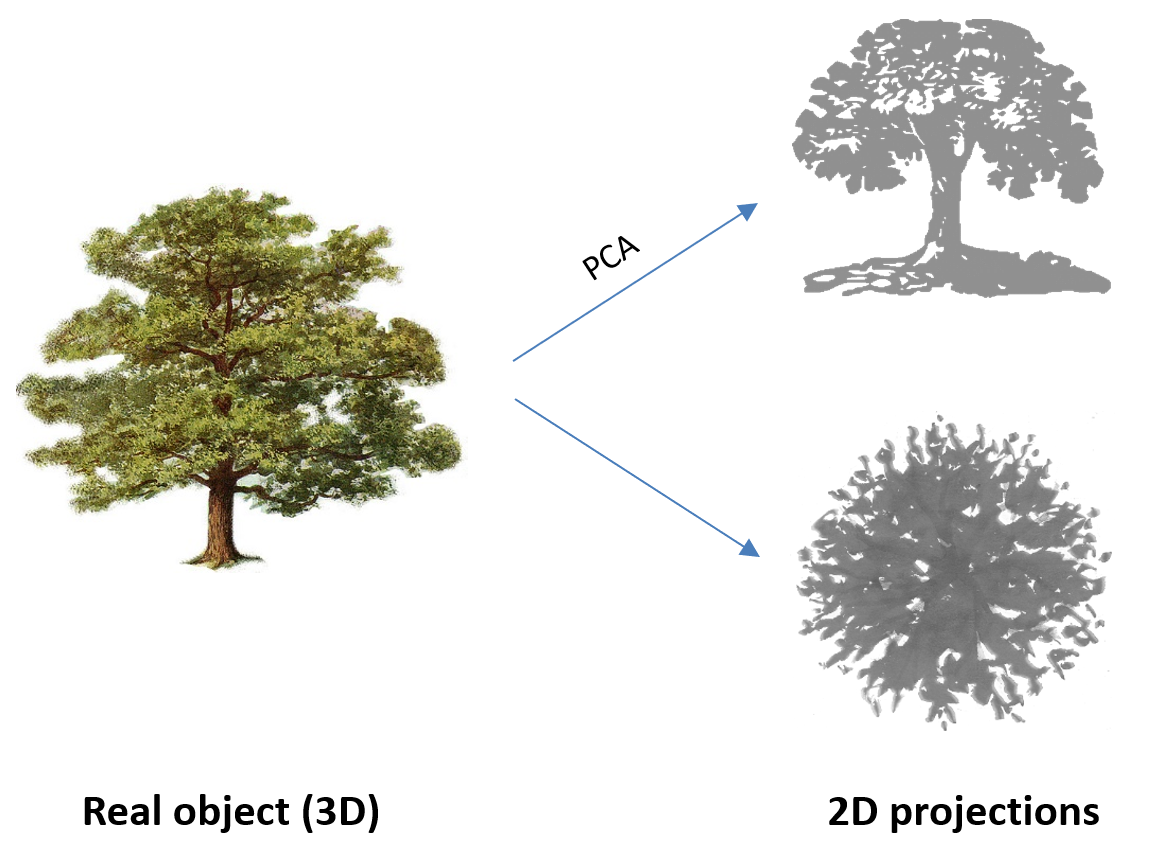
\includegraphics[width=.6\textwidth]{figura02}
		\caption{Variables with less variability can be the ones related to the response, thus being infrarepresented in the first components of PCA. In this example, if we wanted to predict the amount of shadow dropped by the tree, the PCA projection would not be efficient, while the other presented projection fully captures our target prediction. On the other hand, the PCA projection makes the tree fully recognizable, while the other projection makes it hard to even guess there is a tree.}
		\label{figura02}
	\end{figure}

Thus, if the aim is prediction, projection for maximizing the explained variability on the original data matrix is not the best approach. It is much better to maximize covariance with the response. This is how the technique Partial Least Squares (PLS) works.

\subsection{Partial Least Squares}
In linear regression, there is a limit on the number of variables that can enter a model for a specific sample size. Recent studies have shown that a minimum of two independent observations per variable are needed for estimating regression coefficients with reasonable bias \parencite{austin2015number}. Metabolomic data sets usually have many more variables than observations, so linear regression models are not a viable alternative for analyzing these data sets. Linear regression also suffers from multicollinearity, so when highly correlated predictors are used together in a model their coefficients get unstable and standard errors grow wildly \parencite{alin2010multicollinearity}. PLS can be seen as an extension of multiple linear regression designed to overcome the issues just described. It can analyze data sets with strongly correlated variables and handle situations where the number of variables far exceeds the number of observations \parencite{wold2001pls}. Additionally, PLS can also simultaneously model several response variables. It is important to note that results of PLS (and of projection methods in general) depend on the scaling of the data so, before the analyses, the \textbf{X} and \textbf{Y} variables are often scaled to unit variance and centered to the mean.
A scheme of the PLS model is depicted in \autoref{figura17}.

\begin{figure}[hbtp]
	\centering
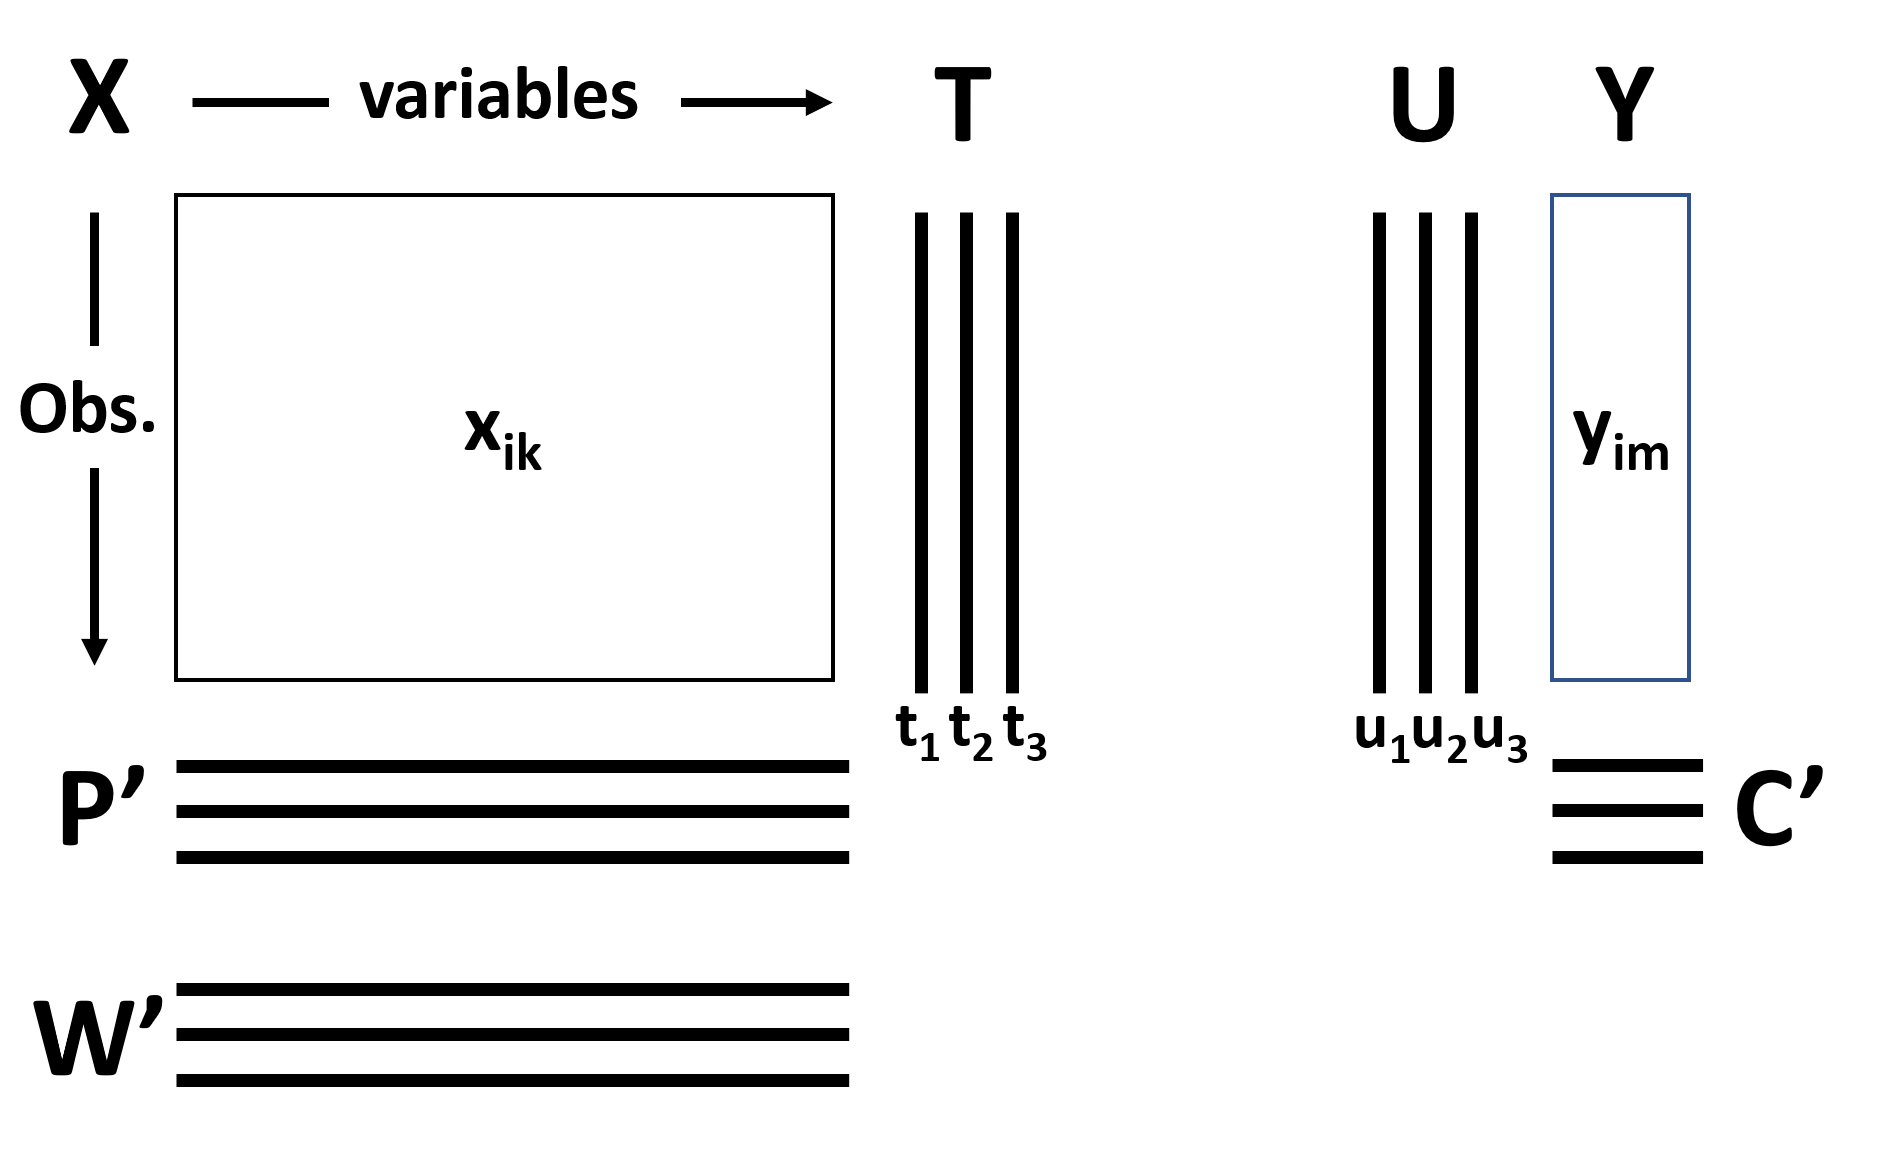
\includegraphics[width=0.7\textwidth]{figura17.png}
\caption{Scheme of the PLS model \parencite{wold2001pls}. \textbf{X} is the matrix of predictors and \textbf{Y} is the matrix of responses. Additional matrices are generated at the different modelling steps.}
\label{figura17}
\end{figure}

The PLS model finds latent variables (denoted by $\text{t}_a$, where a = 1, 2, \dots, A) that are predictors of \textbf{Y} and also model \textbf{X}. These latent variables are also called X-scores and are orthogonal. They are estimated as linear combinations of the original variables using different weights denoted by $\text{w}^*_{ka}$ (\autoref{equation08}). 

\begin{equation}
\label{equation08}
\textbf{\text{T}}=\textbf{\text{XW}}^*
\end{equation}

X-scores are multiplied by the loadings $\text{p}_{ak}$ minimizing residuals in \textbf{X}, denoted as \textbf{E} (\autoref{equation09}).

\begin{equation}
\label{equation09}
\textbf{\text{X}}=\textbf{\text{TP}}'+\textbf{\text{E}}
\end{equation}

Analogously, the Y-scores are multiplied by the weights (denoted by $\text{c}_{am}$) minimizing residuals in \textbf{Y}, denoted as \textbf{G} (\autoref{equation10}).

\begin{equation}
\label{equation10}
\textbf{\text{Y}}=\textbf{\text{UC}}'+\textbf{\text{G}}
\end{equation}

As stated before, X-scores are good predictors of \textbf{Y} (\autoref{equation11}).

\begin{equation}
\label{equation11}
\textbf{\text{Y}}=\textbf{\text{TC}}'+\textbf{\text{F}}
\end{equation}

Where \textbf{F} is the residuals matrix from \textbf{Y}. Alternatively, \autoref{equation11} can be rewritten as follows (\autoref{equation12}):

\begin{equation}
\label{equation12}
\textbf{\text{Y}}=\textbf{\text{XW}}^*\textbf{\text{C}}'+\textbf{\text{F}}=\textbf{\text{XB}}+\textbf{\text{F}}
\end{equation}

Which resembles a multiple linear regression model where the predictors matrix \textbf{X} is multiplied by the coefficients matrix \textbf{B} to predict \textbf{Y}.

With PLS, we have introduced a modelling technique able to effectively deal with metabolomic data. Correlated variables and data sets with many more variables than observations can be properly analyzed and results are easily interpreted with the help of useful plots of the scores, loadings and predictions of the model (\autoref{figura18}).

\begin{figure}[hbtp]
	\centering
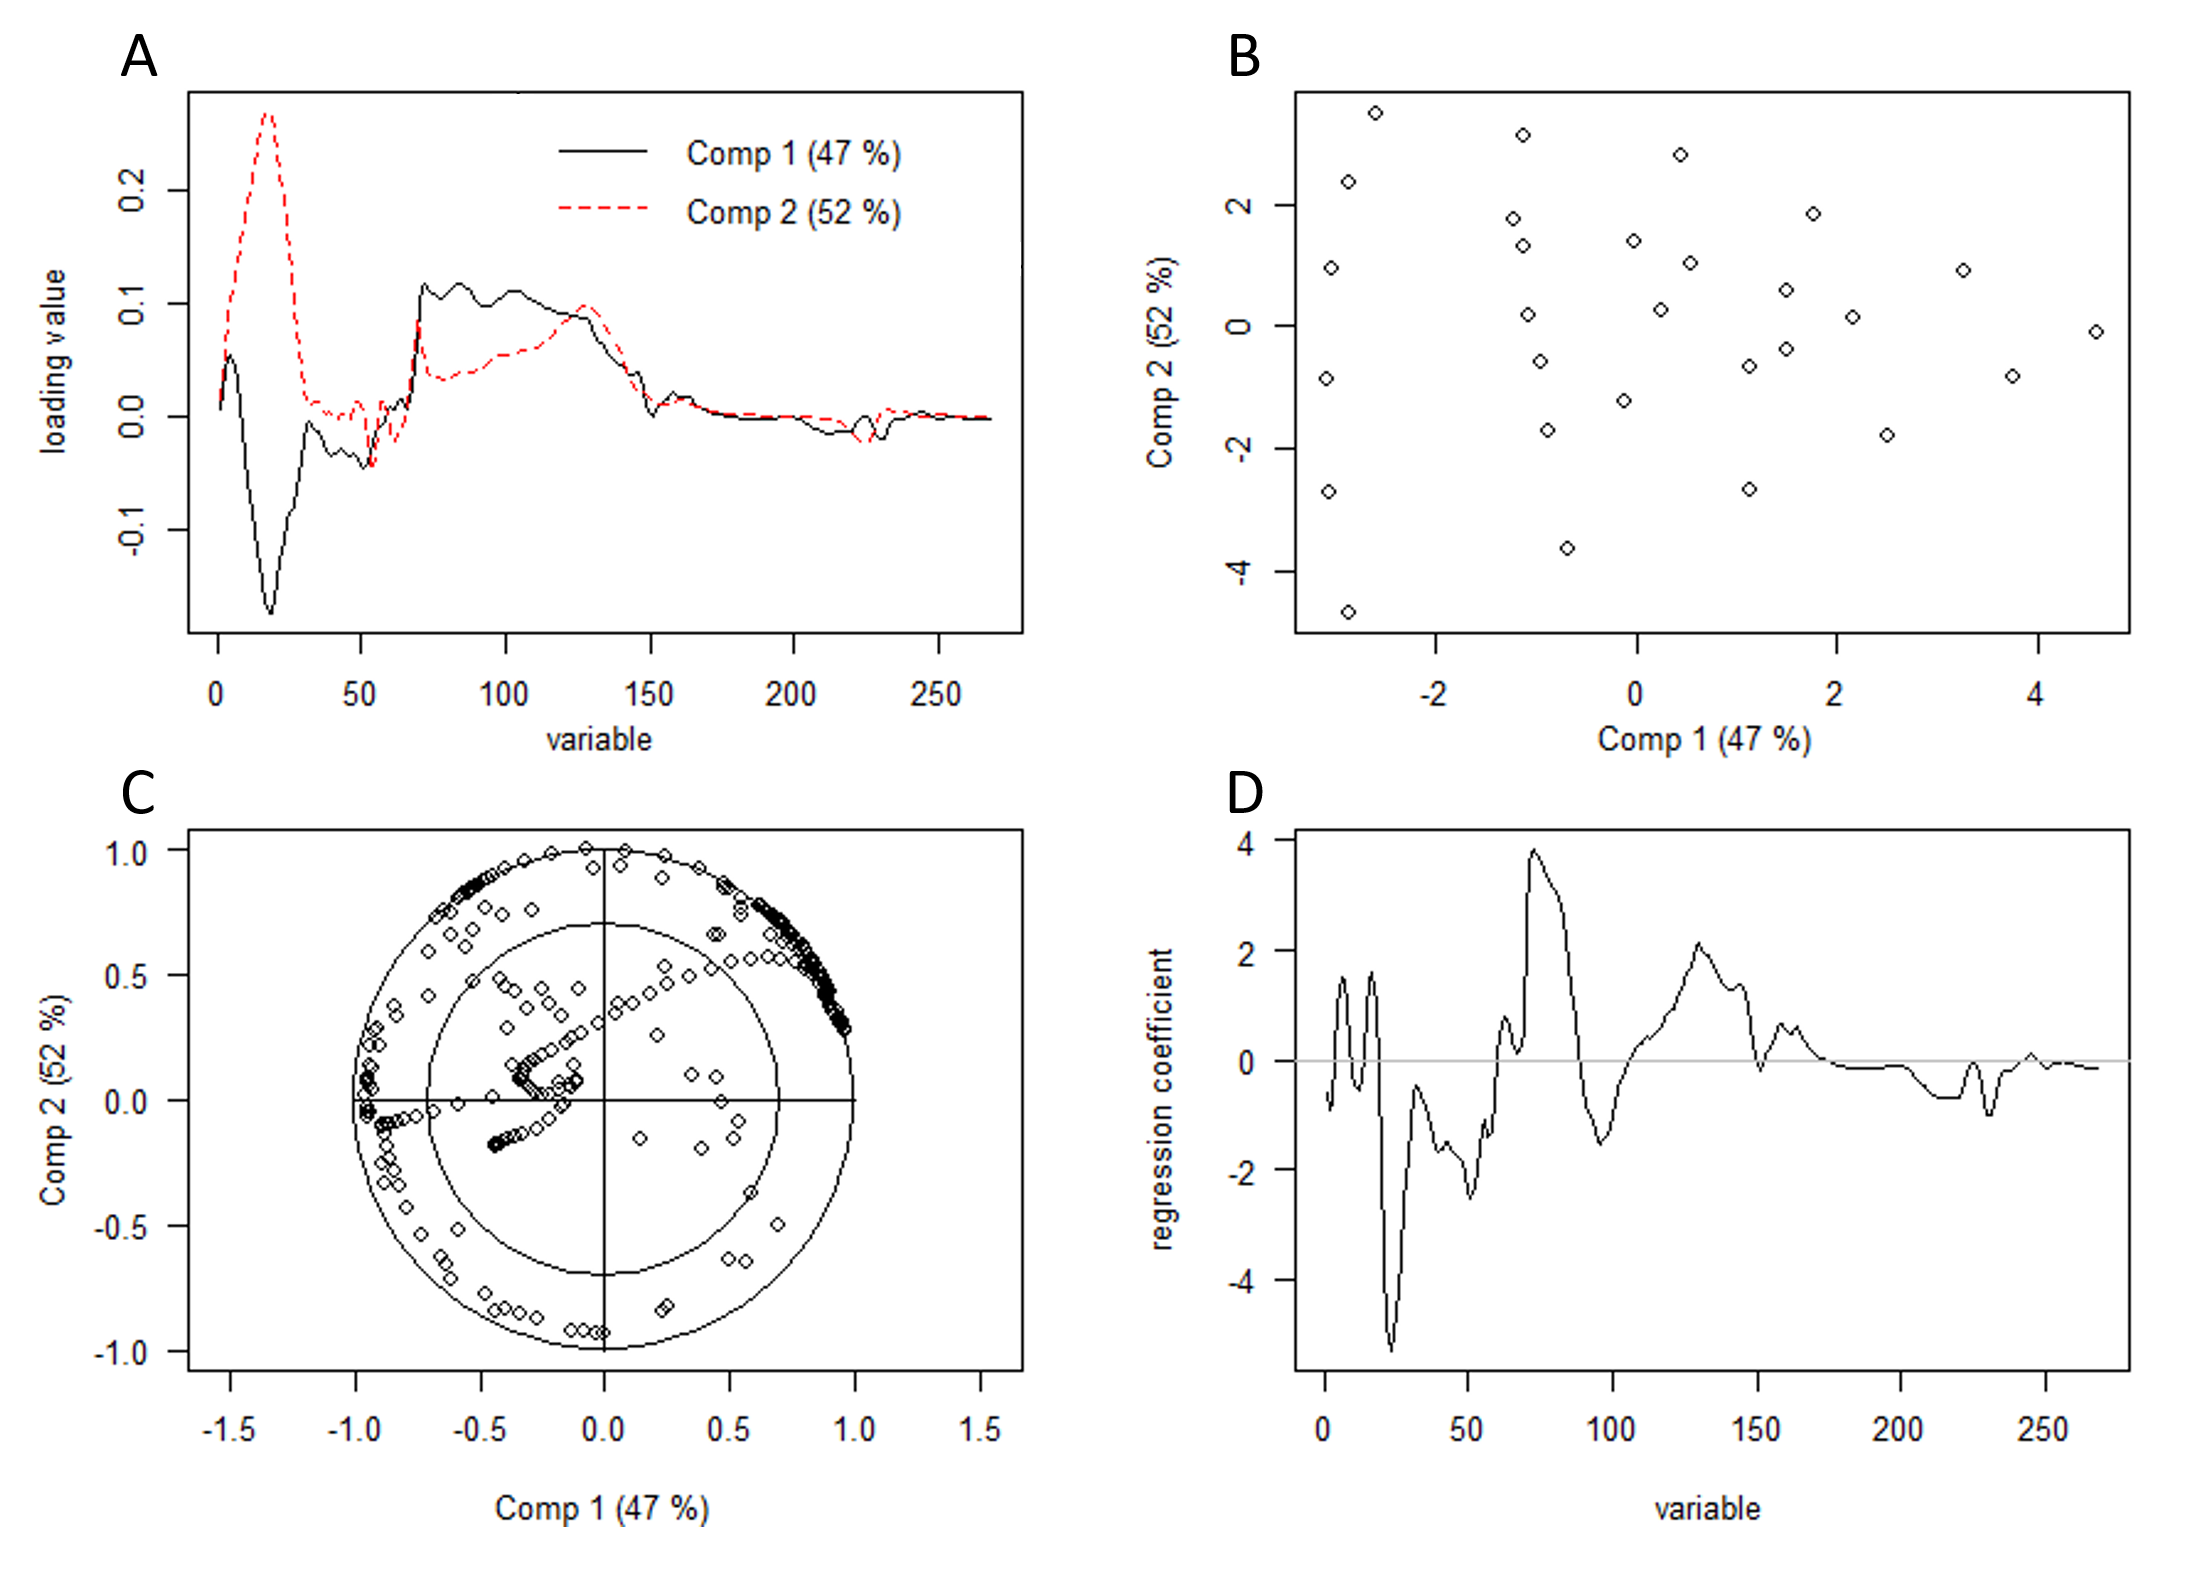
\includegraphics[width=0.82\textwidth]{figura18.png}
\caption{Plots of a PLS model. \textbf{A} shows the loadings for each variable in the two first components. \textbf{B} shows the scores for each observation in the first two components. \textbf{C} represents the correlations between each variable and the first two components.  \textbf{D} shows the regression coefficients of the model.}
\label{figura18}
\end{figure}


\section{Penalization methods}
\label{penalmethods}
Another set of techniques able to deal with metabolomic data sets are the penalization methods. These methods are motivated by the relationship between model complexity and prediction error, also known as bias-variance trade-off \parencite{hastie2001model}. As depicted in \autoref{figura19}, prediction error in the same data set used to fit a specific model always decreases when increasing the complexity of the model. On the other hand, prediction error in new data decreases at first, reaching a minimum at a specific model complexity, and increases later again as model complexity keeps growing larger.

\begin{figure}[hbtp]
	\centering
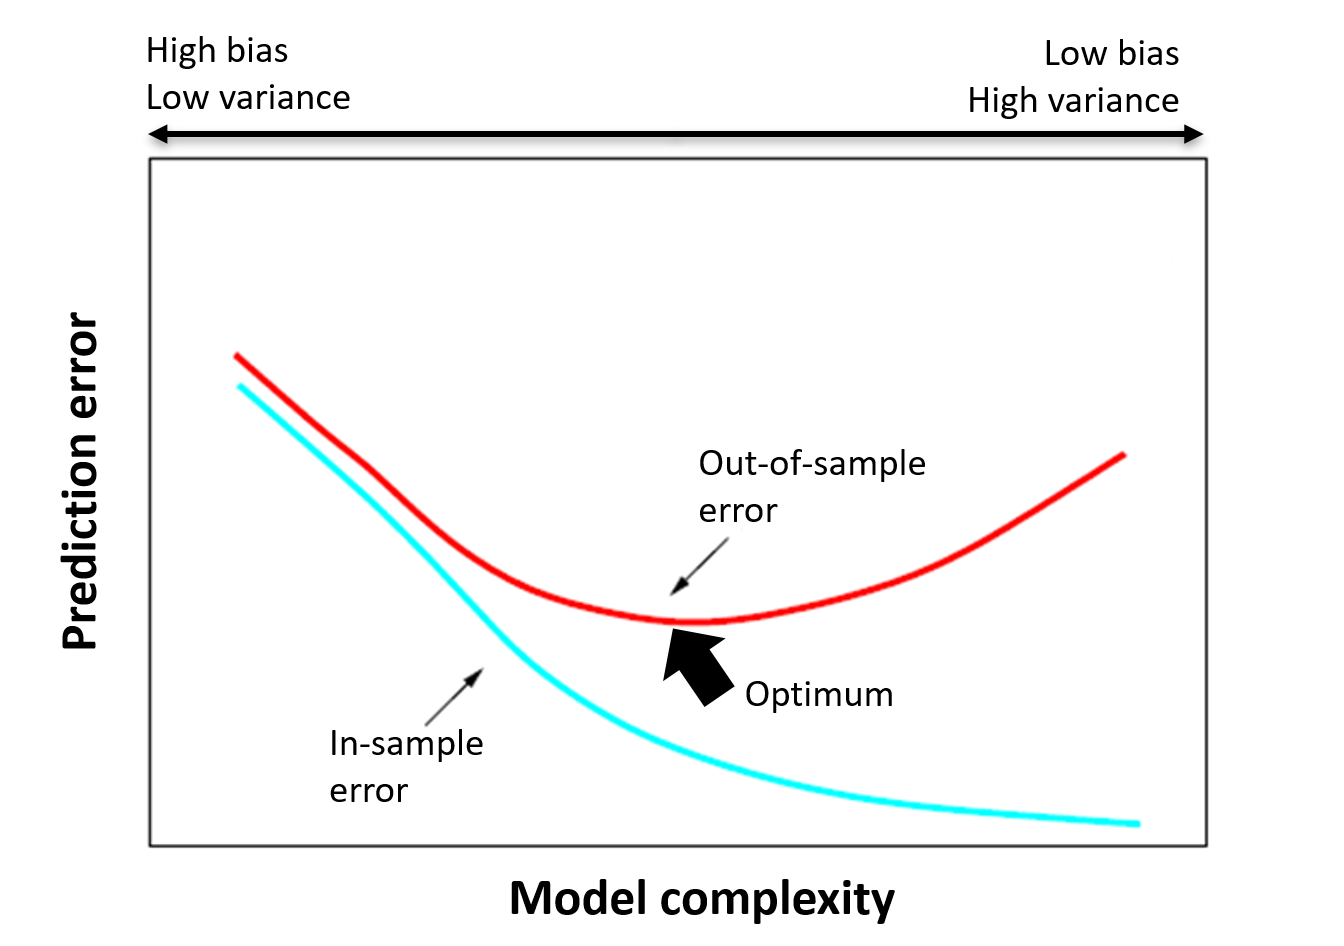
\includegraphics[width=0.75\textwidth]{figura19.png}
\caption{Behavior of prediction error in training (in-sample) and test (out-of-sample) data.}
\label{figura19}
\end{figure}

As previously described, metabolomic data sets are characterized by having a large number of variables and relatively a low number of observations. Trying to fit a model with all the variables in this situation would correspond to the extreme right side of the plot in \autoref{figura19} with low bias and high variance. This is the reason why multiple regression models cannot be fit to these data, variance grows to infinite as the number of predictor variables increases in the model. But this relationship between bias-variance and model complexity gives us the key for improving the standard linear models: increasing bias will reduce the variance, potentially obtaining a lower out-of-sample prediction error because model complexity has been decreased. Thus, the solution for being able to fit linear models to metabolomic data is to bias them. The full reasoning behind this last sentence can be better understood with the explanation provided in \autoref{figura20}.

\begin{figure}[hbtp]
	\centering
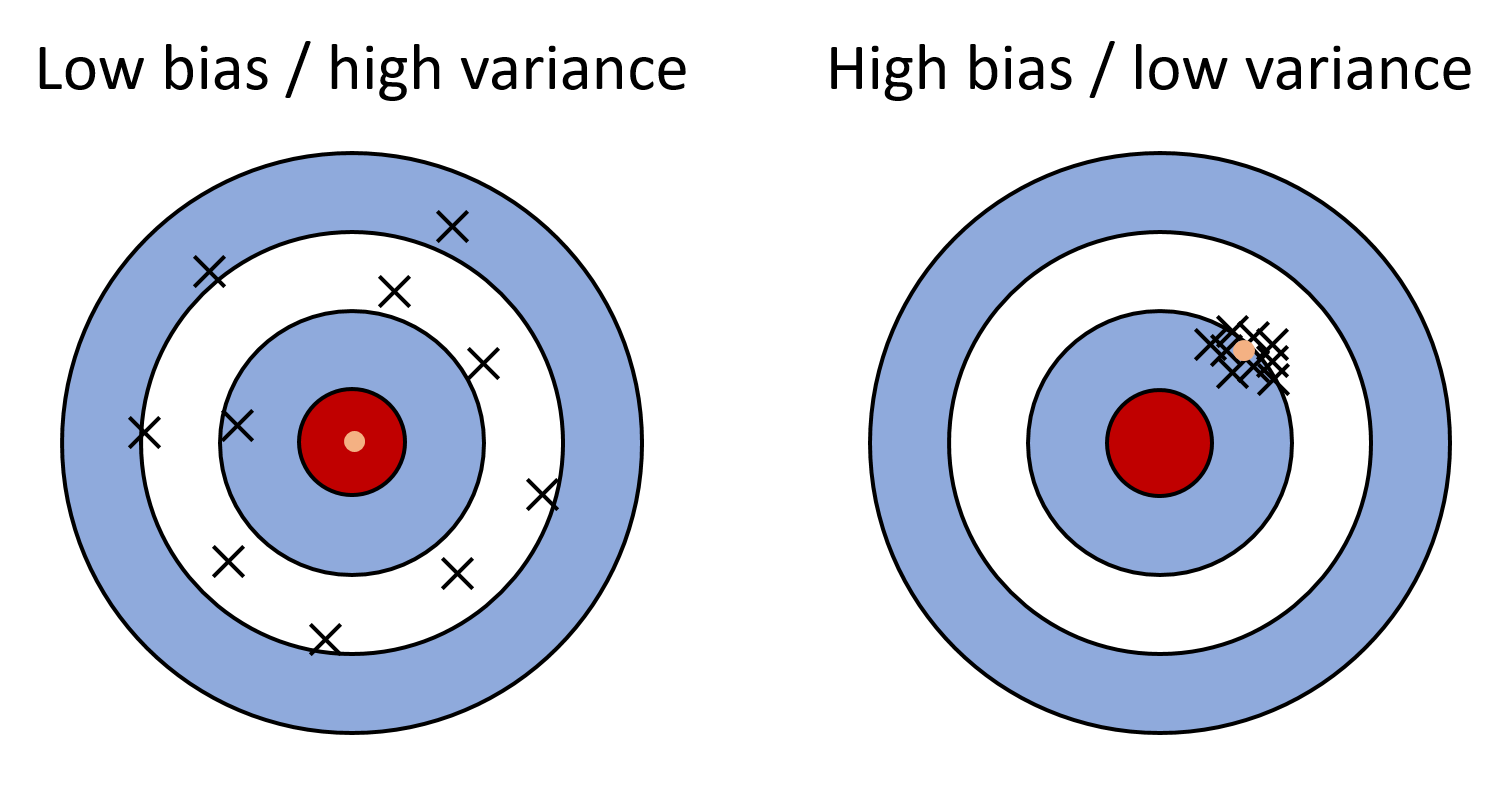
\includegraphics[width=0.75\textwidth]{figura20.png}
\caption{In both targets each black cross represents an estimation of a specific model to different samples of the same population and the orange dot represents the average estimation of all of them. In the left target there is no bias, with the orange dot right at the bullseye, but estimation from the different samples are wildly spread with a very high variability. In the right target, there is a perceptible amount of bias, the orange dot lies out of the bullseye, but all estimations from the different samples are concentrated in a small area around the average estimation. Usually, only one sample (one data set) is available for performing the estimation, so the advantage of introducing bias to lower variance is evident.}
\label{figura20}
\end{figure}

\subsection{Ridge regression}
The first developed penalization method for linear regression was ridge regression \parencite{hoerl1970ridge}. This method consists in solving the ordinary least squares problem, but introduces a restriction to the solution. This restriction consist in setting an upper bound on the sum of the squared coefficients (L2 norm) (\autoref{equation13}).

\begin{equation}
\label{equation13}
\begin{split}
\hat{\beta}^{ridge}=\argmin_\beta \sum\limits_{i=1}^N (y_{i}-\beta_{0}-\sum\limits_{j=1}^p x_{ij}\beta_{j})^{2} \\
\textrm{Subject to the restriction:}  \sum\limits_{j=1}^p \beta_{j}^2\leq s
\end{split}
\end{equation}

The inclusion of this restriction to the ordinary least squares problem imposes a reduction in the value of the coefficients, thus biasing their estimation and producing a reduction in the complexity of the model. A graphical explanation of the functioning of the method is represented in \autoref{figura21}.

\begin{figure}[hbtp]
\centering
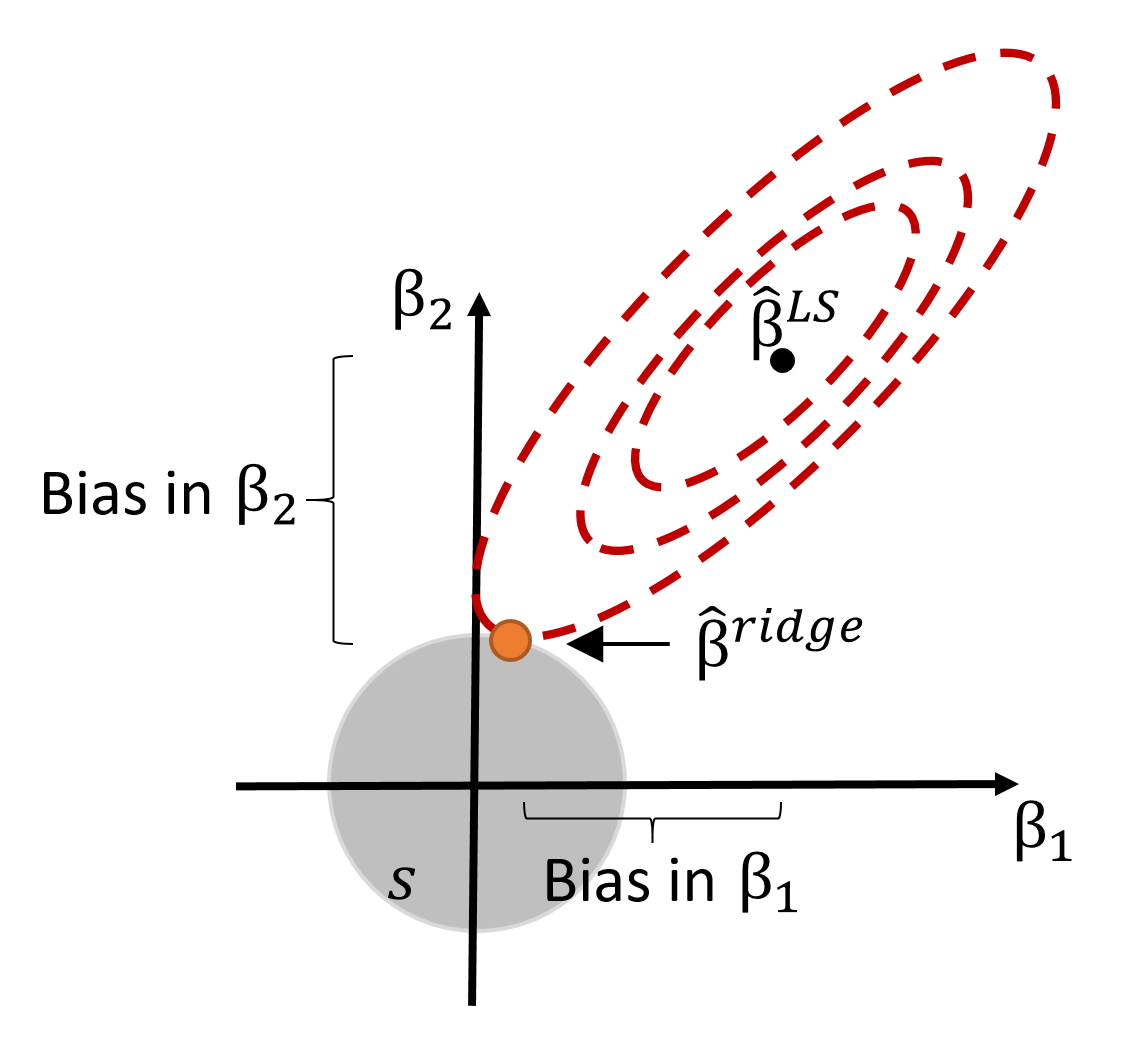
\includegraphics[width=0.6\textwidth]{figura21.png}
\caption{Ridge regression for a linear model with two predictors. As the restriction is intensified (lower value of $s$), the estimation of the coefficients is more biased to zero. Dashed red lines represent least squares contour lines. Grayed area represents the restriction imposed by $s$.}
\label{figura21}
\end{figure}

The solution offered by ridge regression is very similar to that obtained by PLS. A regression model suitable for metabolomic data sets with many, highly correlated variables. Both methods use all the variables for adjusting the model and both models shrink the estimates of the coefficients \parencite{de1995pls}, thus reducing model complexity and therefore variance at a cost of increasing bias.

\subsection{Lasso}
\label{lasso}
In many studies it is the case that it is not only of interest fitting a predictive model, but also selecting the most important predictors among all the variables present in the data. As has been exposed in the previous sections, neither PLS nor ridge regression provide a direct method for variable selection. They both use all the variables in the data set for adjusting the model. It is true that there are some post-model-fitting methods for assessing variable importance in the case of PLS \parencite{mehmood2012review}, but they require and additional filtering step after the model has been fitted and are not inherent to the PLS model. The method known as lasso is similar to ridge regression. But instead of setting a bound on the sum of the squared coefficients, it is set on the sum of the absolute values of the coefficients (L1 norm) as seen in \autoref{equation14} \parencite{tibshirani1996regression}. This change in the method of penalization of the coefficients allows that some of them are set to zero when the model is adjusted, thus producing a variable selection at the model-fitting step.

\begin{equation}
\label{equation14}
\begin{split}
\hat{\beta}^{lasso}=\argmin_\beta \sum\limits_{i=1}^N (y_{i}-\beta_{0}-\sum\limits_{j=1}^p x_{ij}\beta_{j})^{2} \\
\textrm{Subject to the restriction:}  \sum\limits_{j=1}^p |\beta_{j}|\leq s
\end{split}
\end{equation}

\autoref{figura22} shows how increasing the penalization by reducing $s$ forces the parameters to zero, producing a simpler model by deselecting some features. Thus, assuming data are standardized, Lasso automatically selects the most relevant features and discards the others.

\begin{figure}[hbtp]
\centering
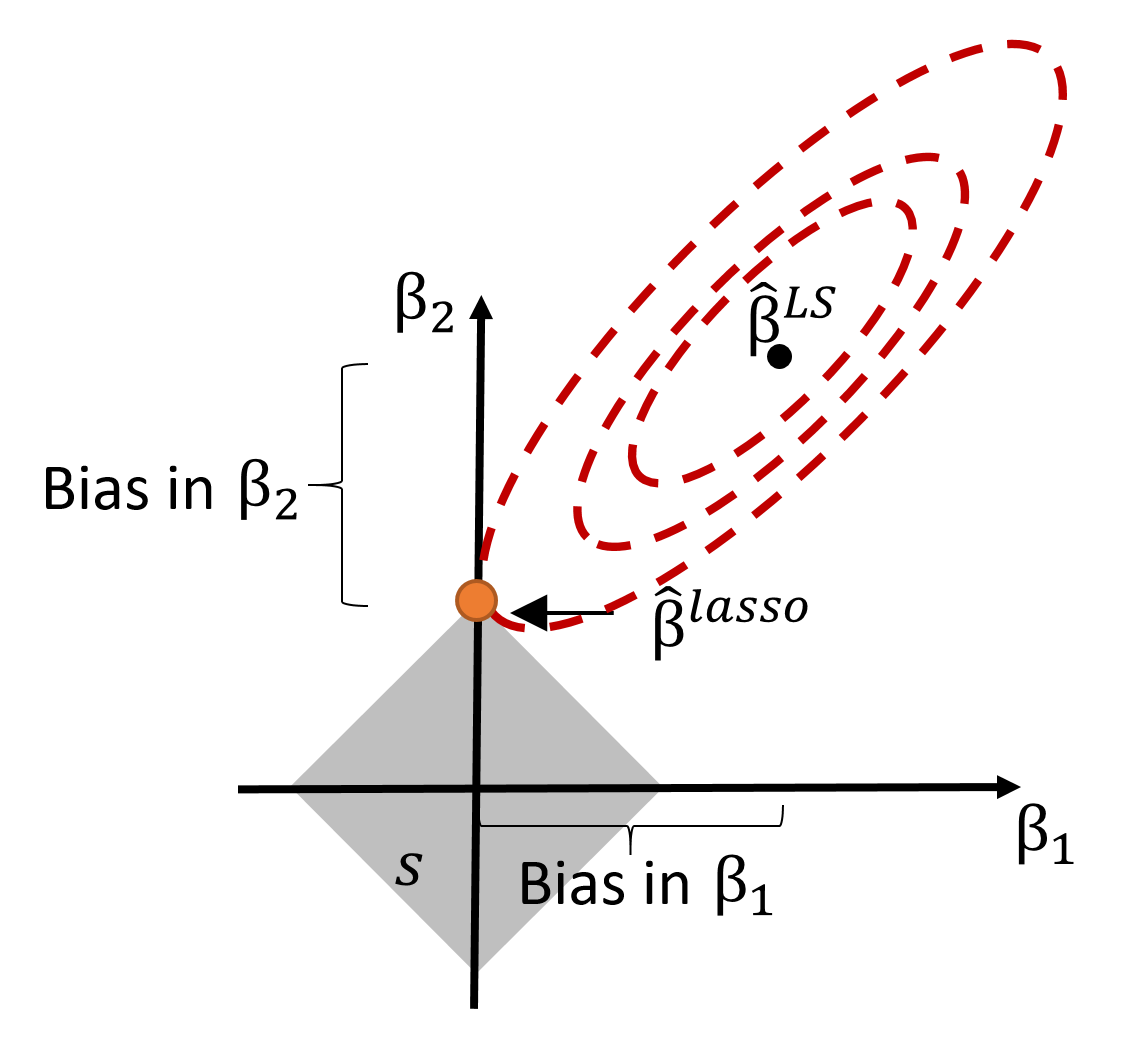
\includegraphics[width=0.6\textwidth]{figura22.png}
\caption{Lasso regression for a linear model with two predictors. As the restriction is intensified (lower value of $s$), the estimation of the coefficients is more biased to zero. Since it is more easier to land in a vertex than in an edge, reducing $s$ forces one of the coefficients to zero. Dashed red lines represent least squares contour lines. Grayed area represents the restriction imposed by $s$.}
\label{figura22}
\end{figure}

The fact that lasso allows for variable selection makes it a very appealing solution for modelling omic data. Unfortunately, unlike PLS and ridge regression, lasso is not able to deal with multicollinearity in an optimal manner \parencite{chong2005performance}, which is a prominent characteristic of metabolimic data. When two (or more) variables are highly correlated, lasso will select one of them discarding the others and, potentially, losing predictive performance and important variables.

\subsection{Elastic net}
Two different penalization methods have been presented, each one with its own benefits and drawbacks. Ridge is able to deal with multicollinearity but does not perform variable selection and lasso performs variable selection but does not deal adequately with multicollinearity. The elastic net algorithm was developed in order to merge the good qualities of ridge and elastic net and overcome their issues \parencite{zou2005regularization}. It is a flexible combination of the two constrains defined for ridge and lasso. The L1 penalty provides variable selection and the L2 penalty provides stability in the selection of correlated variables. The balance between both penalties is defined by the parameter $\alpha$  (\autoref{equation15}). When $\alpha=0$, elastic net is equivalent to ridge regression, since the L1 constraint is set to zero. On the other hand, when $\alpha=1$, elastic net is equivalent to lasso, since the L2 constraint is set to zero. Values between $\alpha = 0$ and $\alpha = 1$ provide different balances between L1 (more variable selection) and L2 (better handling of multicollinearity) penalizations.

\begin{equation}
\label{equation15}
\begin{split}
\hat{\beta}^{elastic net}=\argmin_\beta \sum\limits_{i=1}^N (y_{i}-\beta_{0}-\sum\limits_{j=1}^p x_{ij}\beta_{j})^{2} \\
\textrm{Subject to the restriction: }  \alpha \sum\limits_{j=1}^p |\beta_{j}| + (1-\alpha) \sum\limits_{j=1}^p \beta_{j}^2 \leq s
\end{split}
\end{equation}

\autoref{figura23} depicts the elastic net in a two-variable case and shows how, while keeping the vertices present in lasso, the edges are convex and allow for grouped selection of correlated variables. This is a very attractive solution for the modelling of metabolomic data sets and has been used widely during the last years \parencite{lankinen2010dietary, bowling2014analyzing, liu2015high, ferrario2016mortality}. The only drawback of elastic net compared to lasso and ridge is the inclusion of another parameter in the model. Instead of optimizing only for the value of $s$, elastic net models have also to optimize for the value of $\alpha$, thus requiring more tuning for an appropriate fitting of the data. 

\begin{figure}[hbtp]
\centering
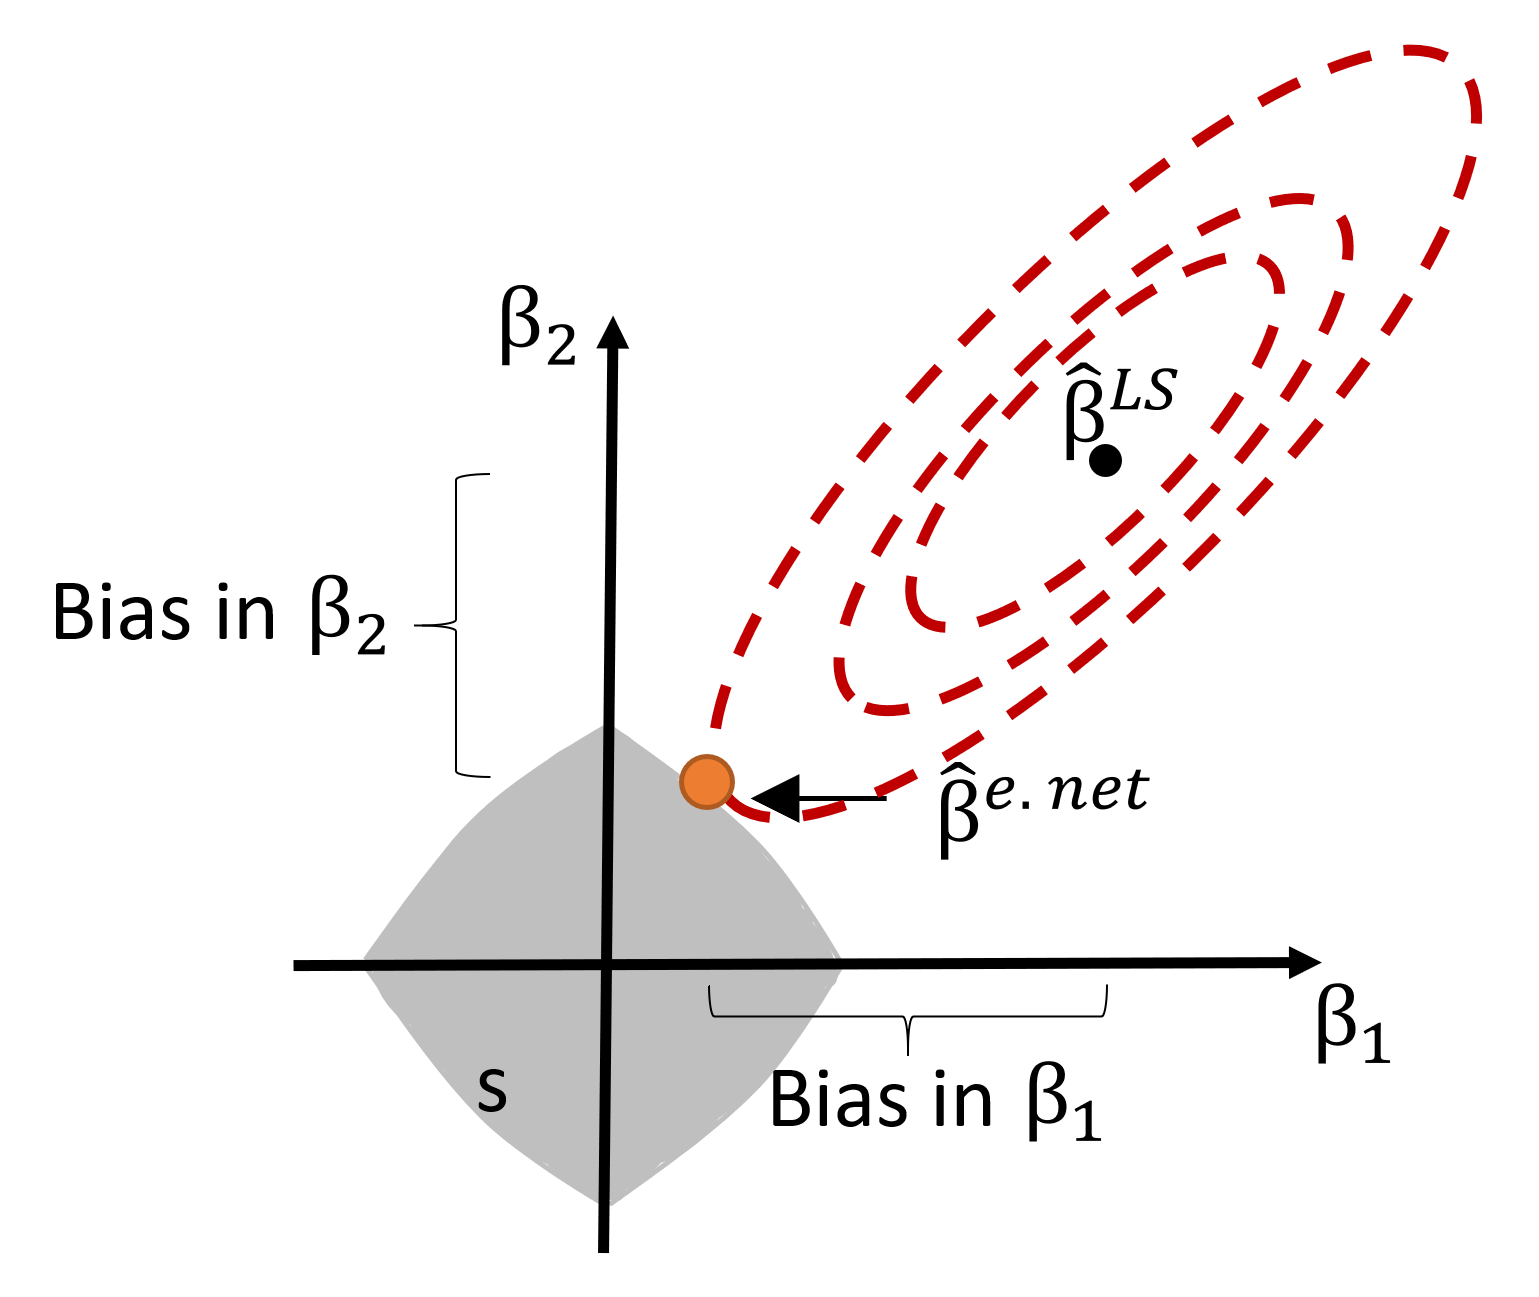
\includegraphics[width=0.6\textwidth]{figura23.png}
\caption{Elastic net regression for a linear model with two predictors. As the restriction is intensified (lower value of $s$), the estimation of the coefficients is more biased to zero. As in lasso, it is more easier to land in a vertex than in an edge, so many coefficients can be potentially set to zero. But, as in ridge, edges are convex, so highly correlated variables will be selected together. Dashed red lines represent least squares contour lines. Grayed area represents the restriction imposed by $s$.}
\label{figura23}
\end{figure}

\section{Tree-based methods}
Projection based methods and penalization methods are extensions of the standard linear model and can also be extended to generalized linear models and survival models without much effort \parencite{nygaard2008partial, simon2011regularization}. But, in essence, they are parametric models, which means that they are sensitive to outliers \parencite{liebmann2010robust, park2016robust} and that they are limited in the types of relationships among variables they can detect. Their validity is also dependent on assumptions that can or cannot be met depending on the population being analyzed. In contrast, tree-based methods are fully non-parametric methods, so they do not have underlying assumptions to be met. They were developed from an algorithmic perspective instead of from an statistical theory perspective, so many of their statistical theoretical foundations where elaborated after their development as data analysis techniques, instead of before, as is usual with most statistical methods \parencite{breiman2001statistical}. The main difference between these two approaches lies in the interpretation of the data generating process. In one case, the data is assumed to be generated by a stochastic data model which we reproduce and use to make the analysis, in the other case the data generating process is treated as unknown and algorithms are generated based in their prediction capability (\autoref{figura24}).

\begin{figure}[hbtp]
\centering
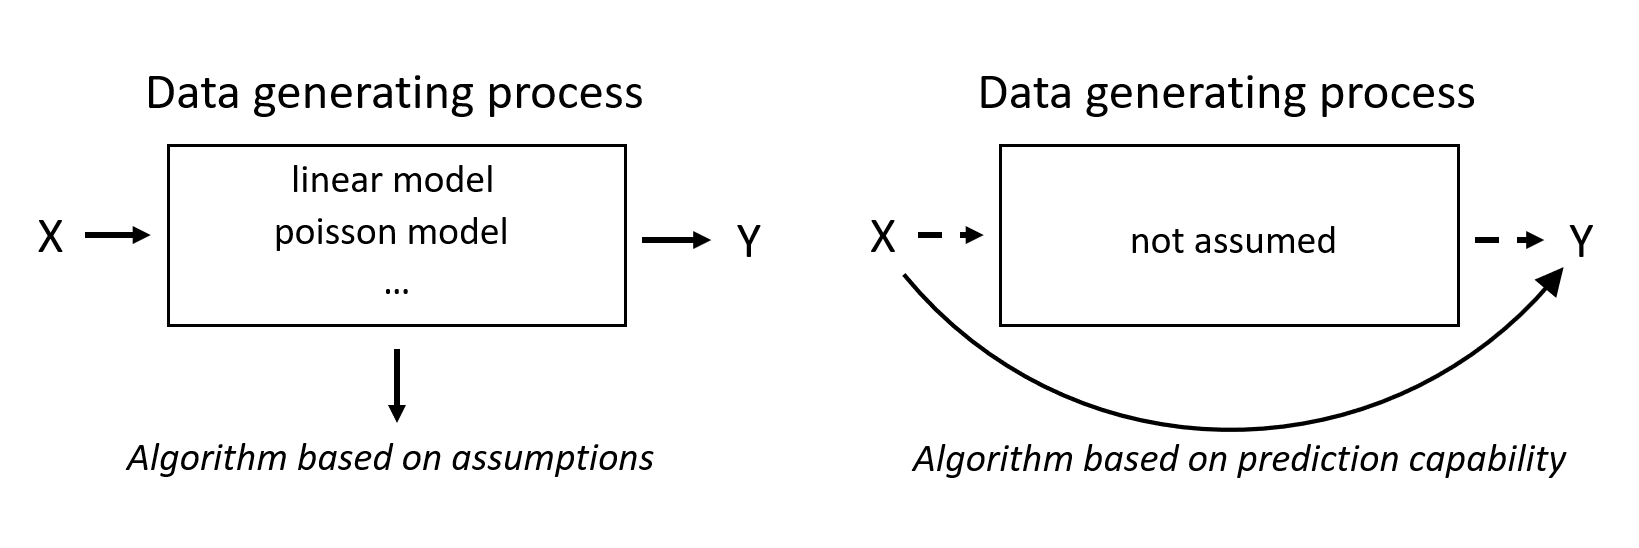
\includegraphics[width=0.9\textwidth]{figura24.png}
\caption{Differences between methods based on assumptions (left) and methods based on predictive capability (right).}
\label{figura24}
\end{figure}

\subsection{Regression and classification trees}
\label{decisiontrees}
Regression and classification trees, also known as decision trees are one of the simplest methods based on trees. They are based on a series of logical decisions structured in a flowchart form, with dichotomic decision nodes based on the different predictor variables. These nodes split into different branches of the tree depending on the decision. The initial node, also called the root node, is at the top of the tree. From there, data passes through various decision nodes until it reaches one of the final nodes of the tree, also called leafs, which contain the prediction of the model. \autoref{figura25} represents a classification tree for predicting relapse in breast cancer. One of the advantages of trees is their ease of interpretation. There is no need of formulas or difficult theory behind them. They are just a flowchart with dichotomic decisions at each node, so all the mechanisms by which a specific prediction is made are fully transparent even for non-experts. They also can deal naturally with categorical predictors and also with missing values and are virtually immune to outliers \parencite{venables2002tree} and to collinearity \parencite{loh2014fifty}. But, in spite of all these strengths, they also suffer from several issues which limit their usefulness when dealing with metabolomic data sets. One of the main issues is their non-smooth bias-variance curve. Small trees are usually too simple, thus underfiting the data (high bias), but they rapidly grow to very complex trees that overfit the data (high variance). This makes it very difficult to achieve a good balance between bias and variance resulting in a good predictive model. For this reason, single decision trees are only used for very simple problems, leaving the complex ones for more sophisticated tree-based methods.

\begin{figure}[hbtp]
\centering
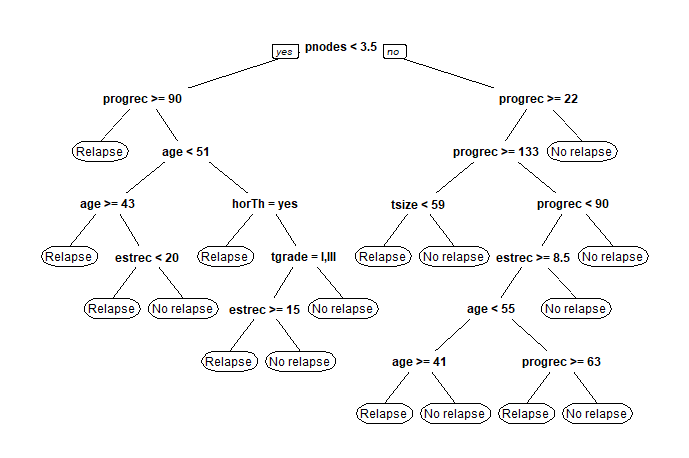
\includegraphics[width=0.9\textwidth]{figura25.png}
\caption{Classification tree for predicting relapse in breast cancer patients. Starting from the top one, each node tests a boolean condition which determines the direction of the next node to test until a terminal node is reached and a prediction is made.}
\label{figura25}
\end{figure}

\subsection{Random forests}
As explained in \autoref{decisiontrees}, single trees are not able to achieve a reasonable balance between bias and variance when adjusting the model. The method known as random forest \parencite{breiman2001random} is inspired in the reasoning behind what was already exposed in \autoref{figura20} of \autoref{penalmethods}. In that figure, there are two targets, the first one corresponding to a zero bias / high variance situation and the second one corresponding to a moderate bias / low variance situation. Since only one sample is usually available (corresponding to just one shot at the target), it is more reasonable to use the moderate bias / low variance target. However, if we had a sufficient amount of large enough samples and could fit one model to each sample, the zero bias / high variance situation would be the best, since averaging the different models would reduce variance and maintain the low bias. This is how random forest works. It creates different instances of the data set using bootstrap resampling \parencite{efron1994introduction} and trains one decision tree to each instance. Since bootstrap samples are correlated, predictor variables are selected at random at each node in each tree to make the models fitted to the different samples more diverse. When performing a prediction, the results of each tree are combined into a single outcome by voting. 

Random forests are among the best methods for predictive modelling, being immune to almost all of the problems commented for the other introduced methods and having very competitive error rates in almost all situations \parencite{fernandez2014we}. Their only drawbacks for its use when analyzing metabolomic data are that they are not easily interpretable and that they do not strictly provide variable selection, although they provide variable importance measures \parencite{archer2008empirical}.

\subsection{Boosting}
As random forest, boosting consists in combining different decision trees to improve prediction accuracy. But, instead of reducing variance like random forest, boosting combines small trees (or any other weak learner) to reduce bias \parencite{freund1996experiments}. The different resampled data sets are generated also differently. In the case of boosting, data sets are generated sequentially in an iterative way. \autoref{figura26} depicts a scheme of how boosting works.

\begin{figure}[hbtp]
\centering
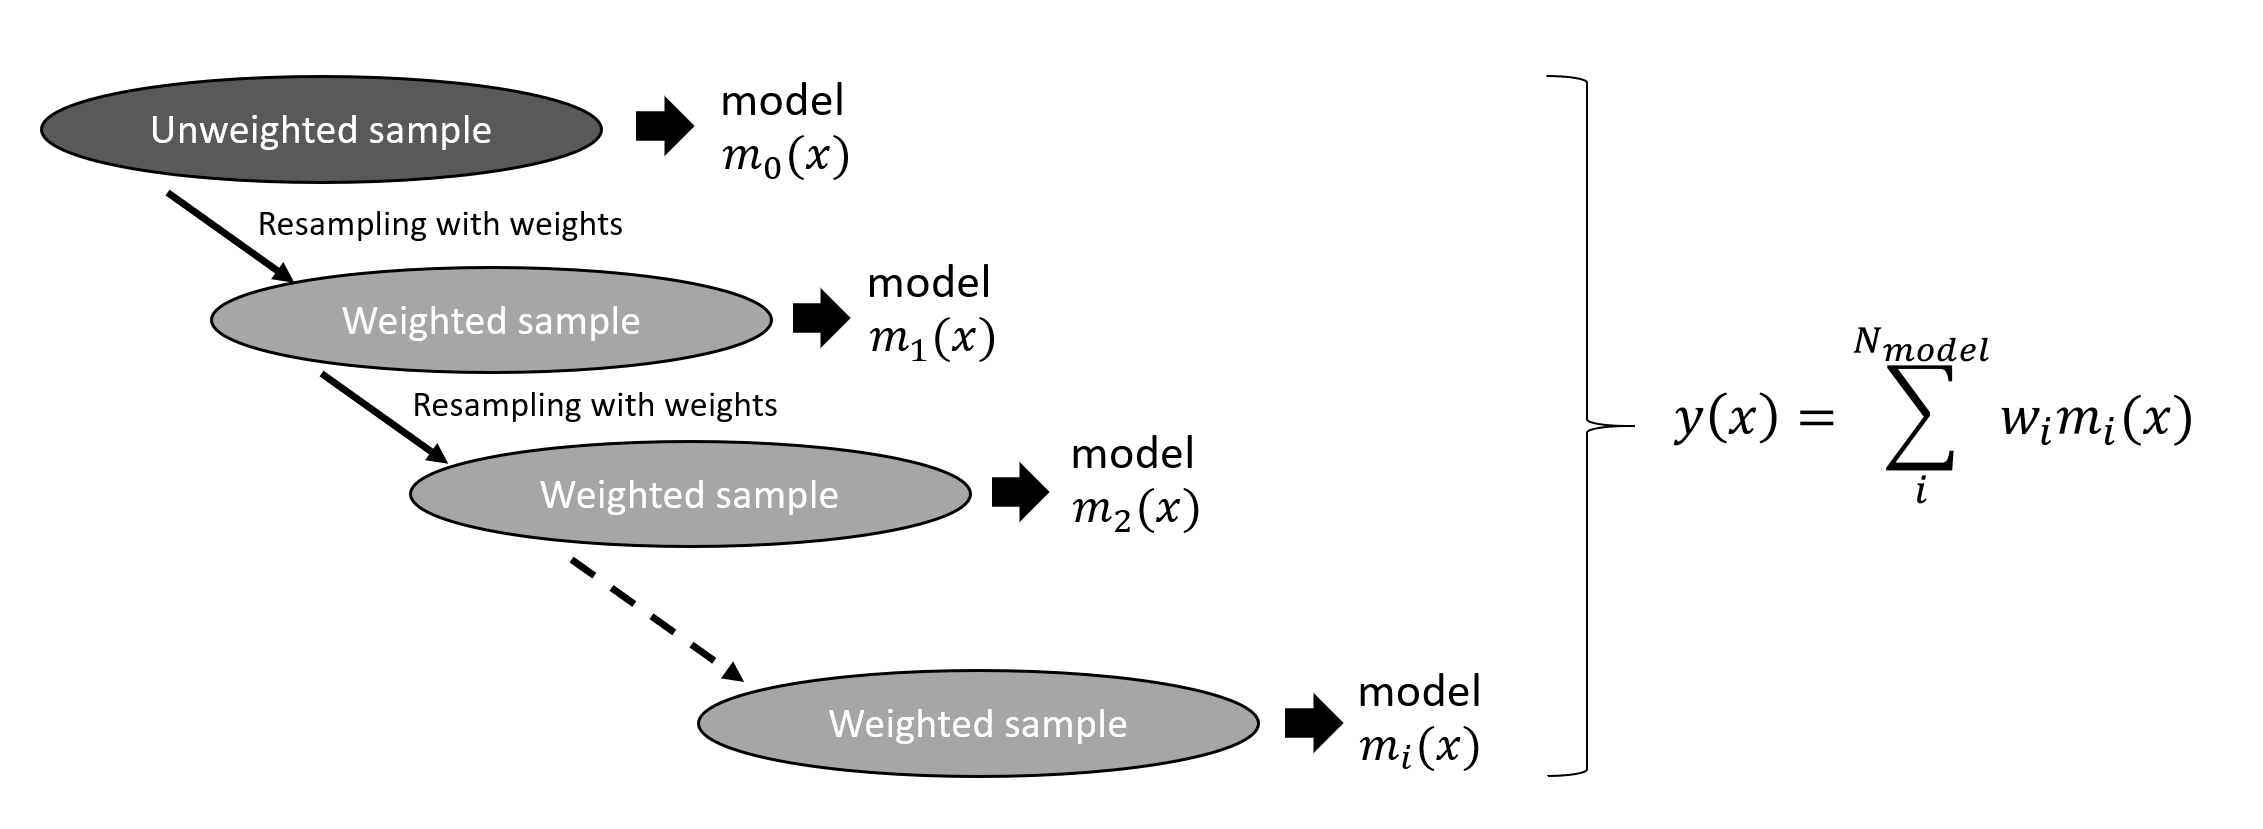
\includegraphics[width=0.85\textwidth]{figura26.png}
\caption{Representation of the boosting algorithm. Each time a model is fitted, a new weighted sample is generated based on the results of the model.}
\label{figura26}
\end{figure}

Beginning from an unweighted data set, the first tree is fitted and a new data set will be generated where observations that were mispredicted will appear more frequently than observations correctly predicted. This way, next model will learn from the mistakes of the previous one, improving prediction error. After this, a new data set will be produced where the mispredicted observations from the second model will be overrepresented compared to the correctly predicted observations. This steps will be repeated until the error rate is low enough. Predictions of the model are estimated using weighted voting based on their accuracy. As random forest, boosting is among the best methods for predictive modelling regarding prediction accuracy, but it suffers from the same issues as random forest regarding interpretability and variable selection \parencite{auret2011empirical}.

\section{Other methods}
Although projection, penalization and tree-based methods have been covered in detail, there are other methods worth mentioning when thinking about dealing with metabolomic data sets. Among them stand out neural networks \parencite{dayhoff2001artificial}, support vector machines \parencite{mahadevan2008analysis} and bayesian networks \parencite{bartel2013statistical}.